% Options for packages loaded elsewhere
\PassOptionsToPackage{unicode}{hyperref}
\PassOptionsToPackage{hyphens}{url}
\documentclass[
]{article}
\usepackage{xcolor}
\usepackage{amsmath,amssymb}
\setcounter{secnumdepth}{-\maxdimen} % remove section numbering
\usepackage{iftex}
\ifPDFTeX
  \usepackage[T1]{fontenc}
  \usepackage[utf8]{inputenc}
  \usepackage{textcomp} % provide euro and other symbols
\else % if luatex or xetex
  \usepackage{unicode-math} % this also loads fontspec
  \defaultfontfeatures{Scale=MatchLowercase}
  \defaultfontfeatures[\rmfamily]{Ligatures=TeX,Scale=1}
\fi
\usepackage{lmodern}
\ifPDFTeX\else
  % xetex/luatex font selection
\fi
% Use upquote if available, for straight quotes in verbatim environments
\IfFileExists{upquote.sty}{\usepackage{upquote}}{}
\IfFileExists{microtype.sty}{% use microtype if available
  \usepackage[]{microtype}
  \UseMicrotypeSet[protrusion]{basicmath} % disable protrusion for tt fonts
}{}
\makeatletter
\@ifundefined{KOMAClassName}{% if non-KOMA class
  \IfFileExists{parskip.sty}{%
    \usepackage{parskip}
  }{% else
    \setlength{\parindent}{0pt}
    \setlength{\parskip}{6pt plus 2pt minus 1pt}}
}{% if KOMA class
  \KOMAoptions{parskip=half}}
\makeatother
\setlength{\emergencystretch}{3em} % prevent overfull lines
\providecommand{\tightlist}{%
  \setlength{\itemsep}{0pt}\setlength{\parskip}{0pt}}
\usepackage{graphicx}
\usepackage{luatexja}
\usepackage{luatexja-fontspec}
\setmainfont{Times New Roman}
\setmainjfont{Yu Mincho}
\setsansjfont{Yu Mincho}
\setmonofont{Yu Mincho}


\usepackage{fancyhdr}
\usepackage{lastpage}
\pagestyle{fancy}
\fancyhf{}
\fancyfoot[C]{\thepage{} / \pageref{LastPage}}

\makeatletter
\renewcommand{\maketitle}{
  \begin{center}
    {\LARGE\bfseries \@title \par}
    \vspace{1em}
  \end{center}

  \begin{flushright}  % 右寄せブロック開始
    {\small \@author \par}              % 著者
    \vspace{0.5em}
    {\small \@date \par}                % 日付
    \vspace{0.5em}\rule{\linewidth}{0.4pt} % 薄い横線
  \end{flushright}  

  }
\makeatother
\usepackage{bookmark}
\IfFileExists{xurl.sty}{\usepackage{xurl}}{} % add URL line breaks if available
\urlstyle{same}
\hypersetup{
  pdftitle={画像テスト},
  pdfauthor={XXXXXX},
  hidelinks,
  pdfcreator={LaTeX via pandoc}}

\title{画像テスト}
\author{XXXXXX}
\date{2025年4月}

\begin{document}
\maketitle

\section{画像テスト}\label{ux753bux50cfux30c6ux30b9ux30c8}

\section{画像レイアウトテスト}\label{ux753bux50cfux30ecux30a4ux30a2ux30a6ux30c8ux30c6ux30b9ux30c8}

\subsection{1枚(縦長画像テスト)}\label{ux679aux7e26ux9577ux753bux50cfux30c6ux30b9ux30c8}

\begin{center}
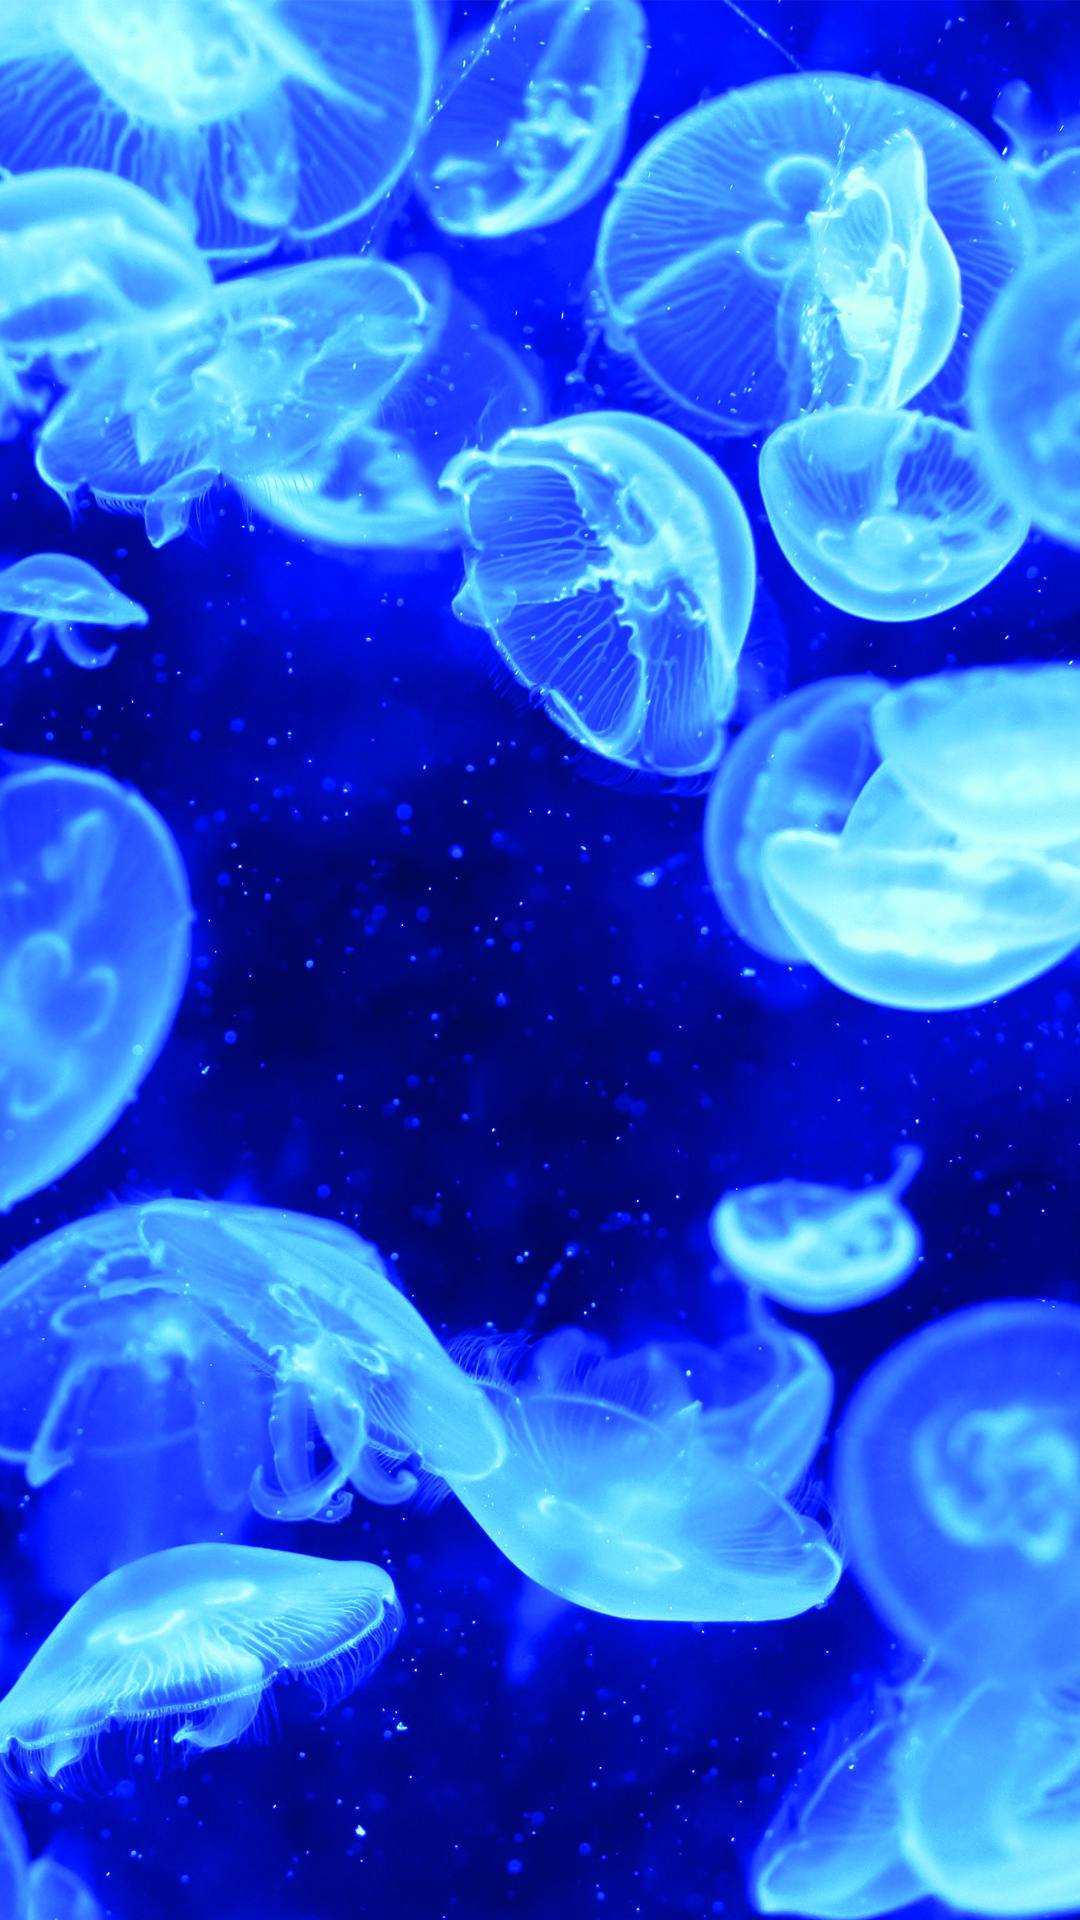
\includegraphics[width=\dimexpr0.60\linewidth\relax,height=0.8\textheight,keepaspectratio]{img/tall.jpg}
\end{center}

以上が1枚のとき(高さ80vh/幅60\%)。

\begin{center}\rule{0.5\linewidth}{0.5pt}\end{center}

\subsection{6枚(折り返しテスト)}\label{ux679aux6298ux308aux8fd4ux3057ux30c6ux30b9ux30c8}

\begin{center}

\includegraphics[width=\dimexpr0.18\linewidth\relax]{img/img1.png}

\includegraphics[width=\dimexpr0.18\linewidth\relax]{img/img2.png}

\includegraphics[width=\dimexpr0.18\linewidth\relax]{img/img3.png}

\includegraphics[width=\dimexpr0.18\linewidth\relax]{img/img4.png}

\includegraphics[width=\dimexpr0.18\linewidth\relax]{img/img5.png}
\end{center}

\begin{center}

\includegraphics[width=\dimexpr0.18\linewidth\relax]{img/img6.png}
\end{center}

→ 最初の5枚は横並び、6枚目は次の行で横並び(1枚扱い)になります。

\begin{center}\rule{0.5\linewidth}{0.5pt}\end{center}

\subsection{通常テキスト}\label{ux901aux5e38ux30c6ux30adux30b9ux30c8}

これはテキストです。

\begin{center}\rule{0.5\linewidth}{0.5pt}\end{center}

\subsection{3枚}\label{ux679a}

\begin{center}

\includegraphics[width=\dimexpr0.31\linewidth\relax]{img/img1.png}

\includegraphics[width=\dimexpr0.31\linewidth\relax]{img/img2.png}

\includegraphics[width=\dimexpr0.31\linewidth\relax]{img/img3.png}
\end{center}

→ 3枚なら1行で均等幅。

\end{document}
